\documentclass[a4paper,12pt, final]{report}
\usepackage{graphicx}
\usepackage{url}
%\usepackage[nomain,acronym,xindy,toc]{glossaries} % nomain, if you define glossaries in a file, and you use \include{INP-00-glossary}
%\makeglossaries
%\usepackage[xindy]{imakeidx}
%\makeindex
%\usepackage[section]{placeins}
\renewcommand\bibname{References}
\usepackage[utf8]{inputenc}
%\usepackage{algorithm2e}
%\usepackage{wrapfig}
\usepackage{epsfig}
%\usepackage{hyperref}
\usepackage[hidelinks]{hyperref} % To Hide the box around links
\renewcommand\bibname{References}
%\usepackage{algorithm2e}
\usepackage{color}
\usepackage{textcomp}
\usepackage{acronym}
\usepackage[top=0.5in, bottom=1in, left=1in, right=1in]{geometry}
\usepackage{xcolor}
\definecolor{dark-red}{rgb}{0.4,0.15,0.15}
\definecolor{dark-blue}{rgb}{0.15,0.15,0.4}
\definecolor{medium-blue}{rgb}{0,0,0.5}

\newcommand{\BigO}[1]{\ensuremath{\operatorname{O}\bigl(#1\bigr)}}
\parindent 8pt
\begin{document}
  \thispagestyle{empty}
  \vspace*{1cm}
  {\centering     
  \textbf{\LARGE Processing In Memory}\\
  \vspace{1.20cm}
  %\it
  %\vspace{.5cm}
  %\rm
  \textbf{\large Dual Degree Stage 1 Report}\\
  \vspace{1cm}
  {Submitted in partial fulfillment of the requirements}\\
  \vspace{0.25cm}
  {for the }\\
  \vspace{1cm}
  \textbf{ Dual Degree Programme}\\
  \vspace{1.50cm}
  {by}\\
  \vspace{0.20cm}
  \textbf{\large Nayan Barhate}\\
  \vspace{0.25cm}
  \textbf{\large (Roll No. 180070037)}\\
  \vspace{1.8cm}
  {Under the guidance of}\\
  \vspace{0.20cm}
  \textbf{\large Prof. Virendra Singh}\\
    \vspace{0.30cm}
  \vspace{1.450cm}
    \begin{figure}[htb]
    \begin{center}
    
\includegraphics[height=1.5in,width=1.5in]{iitblogo.png}
    \end{center}
    \end{figure}

    
  {\textbf{Department of Electrical Engineering}}\\
  {\textbf{Indian Institute of Technology Bombay}}\\
  {\textbf{October 2022}}
 
 }
 
\renewcommand{\abstractname}{Acknowledgement}
\begin{abstract}
I express my gratitude to my guide Prof. Virendra Singh for providing me the opportunity to work on this topic. 
\\\\
\\\\
\\\\
Nayan Barhate\\
Electrical Engineering\\
IIT Bombay\\\

\end{abstract}


\clearpage 
\renewcommand{\abstractname}{Abstract} 
\abstract{
Processing-in-memory (PIM) is rapidly rising as a viable solution for the memory wall 
crisis, rebounding from its unsuccessful attempts in 1990s due to practicality concerns, 
which are alleviated with recent advances in 3D stacking technologies. However, it is 
still challenging to integrate the PIM architectures with existing systems in
a seamless manner due to two common characteristics: unconventional programming
models for in-memory computation units and lack of ability to utilize large
on-chip caches.
}

\tableofcontents
  \addcontentsline{toc}{chapter}{\listfigurename}
  \listoffigures
%  \printglossaries

%\newglossaryentry{ILP}
%{name = ILP,
%description = Instruction Level Parallelism}
\chapter{Introduction}
All computing systems, including cloud and server platforms, desktop computers, mobile and embedded devices, and sensors, rely heavily on main memory. It is one of the primary pillars of any computing platform, along with 1) processing elements (or computational elements), which can include CPU cores, GPU cores, accelerators, or reconfigurable devices, and 2) communication elements, which can include interconnects, network interfaces, and network processing units.

Processing in Memory takes advantage of the ability to implement a wide range of 
general-purpose processing logic in the logic layer of 3D-stacked memory, as well as the 
high internal bandwidth and low latency available between the logic layer and the memory 
layers. This is a more general approach in which the logic implemented in the logic layer 
can be general purpose, benefiting a wide range of applications. Multiple layers of memory
(typically DRAM in pre-existing systems) are stacked on top of each other in a 3D-stacked
memory. Vertical through silicon vias connect these layers together (TSVs). Thousands of 
TSVs can be placed within a single 3D-stacked memory chip using current manufacturing process technologies.

%A simple addition operation when replaced by an atomic addition command inside
%memory gives significant speedup(53\%) to graphs with high number of vertices(5M), but
%the same command gives us a speeddown(upto 20\%) when executed on graphs with low number
%of vertices(62K). This performance degradation is attributed to the observation
%that sometimes the data on which the command was executed is readily available in
%cache. Thus PIM is not always the panacea and the decision of 'to PIM or Not'
%needs to be handled based on the data locality of the operands.
%\begin{figure}[h]
%  \centering
%  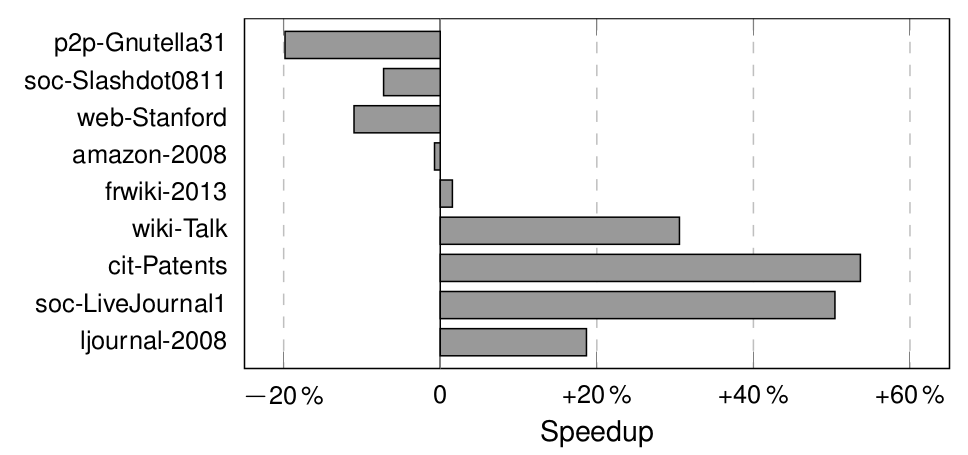
\includegraphics[width=0.8\linewidth]{pim_add.png}
%  \caption{Performance improvement with an in-memory atomic addition operation
%  used for the PageRank algorithm.}
%\end{figure}
\begin{figure}[h]
  \centering
  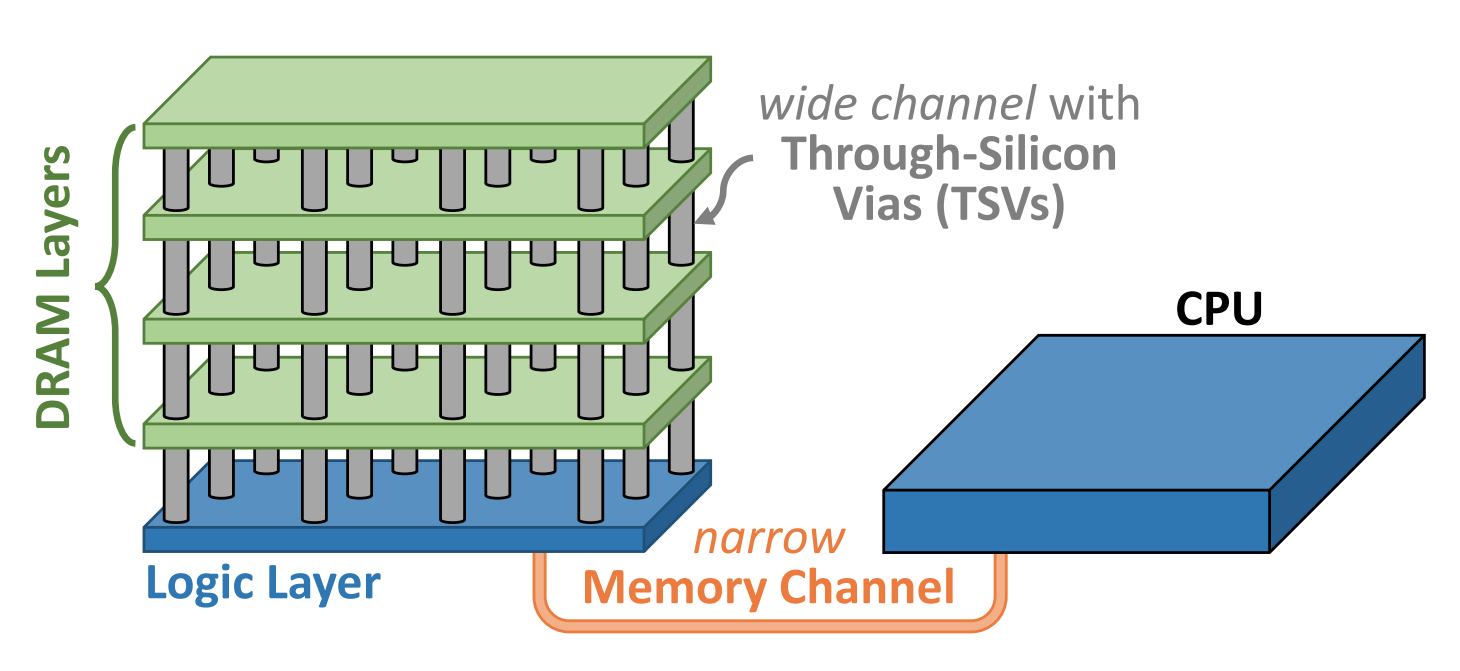
\includegraphics[width=0.8\linewidth]{3dmem.png}
  \caption{High-level overview of a 3D-stacked DRAM architecture\cite{3dmem}}
\end{figure}

\chapter{Literature Survey}
Processing in memory (PIM) involves adding or integrating PIM logic (e.g., accelerators,
simple processing cores, reconfigurable logic) close to or inside the memory. 
Many of these works place PIM logic inside the logic layer of 3D-stacked
memories (eg. Hybrid Memory Cube or HMC)
This PIM processing logic, which we also refer to as PIM cores or PIM engines, 
interchangeably, can execute portions of applications (from individual instructions to 
functions) or entire threads and applications, depending on the design of the architecture. 
Such PIM engines have high-bandwidth and low-latency access to the memory stacks that are 
on top of them, since the logic layer and the memory layers are connected via high-bandwidth 
vertical connections, e.g., through-silicon vias. Systems make use of relatively simple 
PIM engines within the logic layer to avoid data movement and thus obtain significant 
performance and energy improvements on a wide variety of application domains.

\section{Coarse-Grained Application-Level PIM offload}

In coarse grained application PIM offload an entire application is re-written to
completely execute on the PIM substrate. In such a coarse-grained
(i.e., application-granularity) approach,  specialised
programming model and specialised architecture/hardware are required. Large-scale graph
processing is a popular application coarse grained PIM offload. Because of (1) large amounts of
random memory accesses across large memory regions and (2) very small amounts
of computation per data item fetched from memory. Thus graph analysis workloads are
known to put significant strain on memory bandwidth.

Tesseract\cite{tesseract} is an example of a coarse-grained application level PIM accelerator.
Tesseract consists of (1) a new hardware architecture that effectively uses the
available memory bandwidth in 3D-stacked memory by placing simple in-order
processing cores in the logic layer and allowing each core to manipulate data
only on the memory partition it is assigned to control, and (2) an efficient
method of communication between different in-order cores within a 3D-stacked
memory that allows each core to request computation on data elements that
reside in the memory partition it is assigned to control.


Rather than moving data elements across different memory partitions and cores,
the Tesseract design moves functions (i.e., computations and temporary values)
to data that is to be updated. It also includes two hardware prefetchers
specialised for graph processing memory access patterns, which operate based on
hints provided by programming model. 
Tesseract PIM architecture improves average system
performance by 13.8x and achieves an 87\% average energy reduction over conventional systems.

Application can also be offloaded by considering qualitative benefits of PIM such as

parralelizability\cite{inmemmap51}, reduced memory
latency\cite{pointerchasing32}, 
bandwidth savings\cite{tom31}, energy efficiency\cite{energyefficient40}, thermal 
constraints\cite{coolpim47}, and workload characteristics\cite{fafnir12}.  

\section{Fine-Grained Instruction-Level PIM offload}
With Fine grained approach,
individual instructions can be offloaded to the PIM engine and accelerated.
This fine-grained approach can have significant benefits in terms of potential adoption 
since existing processor-centric execution models already operate (i.e., perform computation) 
at the granularity of individual instructions and all such machinery
can be reused to aid offloading to be as seamless as
possible with existing programming models and system
mechanisms. 

PIM-Enabled Instructions (PEI)\cite{PEI_ISCA} aims to provide the minimal processing-in-memory 
support to take advantage of PIM using 3D-stacked memory, in
a way that can achieve significant performance and energy benefits without changing the 
computing system significantly. PEI incorporated a locality-aware mechanism
which tracked the locality of operand and dynamically decides where to execute
the instruction. Examples of PEIs are integer increment, integer minimum, floating-point 
addition, hash table probing, histogram bin index, Euclidean distance, and dot
product. The instructions were tailored to accelarated the application but were distinct 
from the host ISA. This affects significantly in the adoption of PIM for general
purpose processing. Data locality is a great parameter for deciding the
location of execution (host CPU or memory), but is not sufficient. In case the
instruction was executed on the host CPU and one operand from memory, the feteched operand
from memory may not be referenced again and pollutes the cache with unnecessary data movement.


\subsection{Effects of Instruction-level offload}
%All of the above mentioned methods take deceision based on past access with no
%consideration of future. 
In case of PEIs the decision of fetching an operand
from memory can result in pollution of cache. Thus we propose to take decide
the location of execution by considering the affter-effects of fetching operand from
memory / flushing the cacheline from host. Thus we predict the reuse distance
of the cacheline in which the operand resides.  

\chapter{Project Proposal}
Instruction granularity does not affect the programmers model, and thus helps
in the adoption of PIM for general purpose processing. We thus intend to
accelarate X86 SIMD instructions which benefits from execution in PIM engines. For
every operand that needs to be fetched from memory we predict its reuse
distance. This prediction is very similar to mockingjay's\cite{mockingjay} Reuse Distance
Predictor with the difference that the prediction is done for operands of
potential PIM instruction instead of incoming cacheline. If the predicted reuse
distance is greater than any of the reuse distance stored in our predictor, we
mark the instruction an offloadable instruction as fetching the operand from
main memory results in pollution of cacheline and does not help the CPU for further 
operations. 

\bibliographystyle{ieeetr}
\bibliography{thesisTemplate}{}














\end{document}
